
\documentclass{report}


%Marginie interlinea
\usepackage[top=1in, bottom=1in, left=1.2in, right=1in]{geometry}
\pagestyle{plain}
\linespread{1.3}

%Librerie utili
\usepackage[utf8]{inputenc}
\usepackage{libertine}
\usepackage{graphicx}
\usepackage{floatflt}
\usepackage{blindtext}
\usepackage{enumitem}
\usepackage{amsthm}
\usepackage{subfig}
\usepackage{listings}
\usepackage{listingsutf8}
\usepackage{amsmath}
\usepackage{framed}
\usepackage{minibox}
\usepackage{float}
\usepackage{wrapfig}
\usepackage{longtable}
\usepackage[strict]{changepage}
\usepackage{pgfplots}
\usepackage{tikz}
\usetikzlibrary{matrix}
\pgfplotsset{width=11cm,compat=1.9}
\usepgfplotslibrary{external}
\tikzexternalize
\usepackage[colorinlistoftodos]{todonotes}
\usepackage[colorlinks=true, allcolors=black]{hyperref}
\usepackage{caption}
\usepackage{subfigure}
\usepackage{sectsty}
\usepackage{titling} 
\usepackage{xcolor}
\definecolor{darkgreen}{rgb}{0.0, 0.4, 0.0}
\usepackage[Sonny]{fncychap}
\usepackage{lipsum}
\usepackage{apacite}
\usepackage{tabularx}
\usepackage{caption}
\usepackage{subcaption}

\begin{document}
\title{GAN}
\author{Ying Ting (Rhea) Lau
\date{\today}

\begin{titlepage}

\begin{center}
\textsc{ \LARGE{Joint Master's in Applied Geophysics\\}}
\vspace{10mm}

\includegraphics[width=0.3\textwidth]{Figure/Front_page/IDEA_League_Logo.png}
\vspace{5mm}\\
\textsc{ \large{Delft University of Technology, The Netherlands\\ }}
\textsc{ \large{ETH Zürich, Switzerland\\ }}
\textsc{ \large{RWTH Aachen, Germany\\ }}
\vspace{25mm}
\textnormal{ \LARGE{Research Module Report\\}}
\vspace{5mm}
% \fontsize{10mm}{7mm}\selectfont 
% \textup{Generative Adversarial Networks on Traces Interpolation}\\
\textnormal{\huge{Image Reconstruction using \\Generative Adversarial Networks\\}}
\vspace{5mm}
\textnormal{\large{written by\\}}
\textnormal{\Large{Ying Ting (Rhea) Lau\\}}
\vspace{25mm}
\setlength{\columnsep}{500pt}
\begin{tabular}{cccc}
\textbf{\large{External Supervisors}} & & & \textbf{\large{Internal Supervisor}} \\
\textbf{\large{from SLB UK}} & & & \textbf{\large{from ETH Zürich}} \\\\
\large{Dr. Rajiv Kumar} & & & \large{Dr. Dirk-Jan van Manen} \\
\large{Dr. Massimiliano Vassallo} &  \\
\end{tabular}
\end{center}

\vspace{20mm}

\centering{\large{Academic year 2023/2024 \\ \today}}
\end{titlepage}

\chapter*{Abstract}\label{ch:0}
\thispagestyle{empty}
This study focuses on exploring the applicability of deep learning, particularly Generative Adversarial Networks (GANs), on the seismic trace interpolation problem. We first compare conventional seismic interpolation methods with the machine learning counterpart. Subsequently, we evaluate the performance of GANs in the context of image reconstruction, leveraging simplified datasets. Given the complexity and computational demands of seismic datasets, we opted to simulate the seismic problem using the more manageable 28x28 pixel MNIST and Fashion-MNIST datasets. These datasets were augmented by introducing masked columns, mimicking the missing trace scenario encountered in seismic data. We employ three GANs, namely Linear model, LeNeT-5, and U-NET, to reconstruct MNIST and Fashion-MNIST images. Our evaluation involves qualitative assessments and examination of losses. Notably, U-NET emerges as the most effective, producing high-definition results closest to the original images, as evidenced by MSE losses. Through this approach we gained insights into the effectiveness of GANs in handling image reconstruction and their potential in addressing seismic trace interpolation. However, challenges like training instability and feature loss due to missing information highlight the need for further model and hyper-parameters refinement in handling larger and more complex dataset.
\\\\

\tableofcontents
\thispagestyle{empty}
\clearpage 
\setcounter{page}{1} % Reset page number to 1

\chapter{Introduction}\label{ch:intro}
In signal processing, we follow the Nyquist rate $f_{Nyq}=\frac{1}{2\Delta t}$ in sampling signals in order to avoid aliasing. However, sampling at least twice the maximum signal frequency could lead to high surveying and time costs. There are two approaches to address this challenge: compressive sampling and data interpolation. Compressive sampling (CS) leverages the principles of sparsity, which relates to the signals of interest, and incoherence, which relates to the sensing modality \cite{candes2008introduction}. CS theory allows accurate recovery of signals from a significantly reduced set of samples, compared to the traditional Nyquist rate, by sampling only $O(S\log{(n/S)})$ projections. \cite{candes2008introduction} In this study, our focus is on interpolation methods. These methods spatially transform irregularly sampled traces to any desired grid \cite{kaur2021seismic}. There are two major categories of seismic interpolation methods: wave equation methods and signal processing methods \cite{naghizadeh2011seismic,kaur2019seismic,kaur2021seismic}.
\\\\
Wave equation methods are based on seismic wave propagation, which requires prior knowledge of the direction of lateral coherence of the event. A velocity model is a prerequisite for interpreting traces \cite{ronen1987wave}. Given an accurate velocity model, wave-equation-based approaches can interpolate waves passing through complex geological structures and subsurface heterogeneities. Parabolic and hyperbolic events can be recovered. However, subsurface velocity models might not be present for the surveying area. These methods also employ a straight-raypath approximation, which might collapse for low-frequency waves \cite{stolt2002seismic}.
\\\\
Signal processing methods include domain transform methods or prediction filter methods. No subsurface information is required to perform traces interpolation. Multiple studies have outlined other benefits of using signal processing methods: F-X domain interpolation is insensitive to random noises \cite{spitz1991seismic}, F-K domain interpolation can preserve amplitude and perform artifact-free denoise \cite{naghizadeh2011seismic}, fast generalized Fourier transform (FTFG) can handle non-stationary seismic data \cite{naghizadeh2012seismic}, and 3D sparse time-domain Radon interpolator (TDRI) can reconstruct events with high continuity \cite{schonewille2014comparison}. The major drawback is the sparsity and linearity assumptions in the t-x domain, making these methods intolerant to highly curved or dispersed events \cite{spitz1991seismic, naghizadeh2011seismic, naghizadeh2012seismic}.
\\\\
Deep learning methods come without the aforementioned assumptions, and they do not require any velocity model. Convolutional neural networks (CNNs) combine domain transforms and prediction filter methods but without the linearity assumptions or time/frequency transforms \cite{oliveira2018interpolating}. Transforms and filters are learned and applied to the neural networks through an iterative training process. Figure \ref{fig:methods} shows different algorithms that have been exploited for seismic traces interpolation, such as CNNs, generative adversarial networks (GANs), and auto-encoders \cite{khosro2023machine}. These deep learning methods yield high reconstruction accuracy even on steep events and can be easily applied to 3D data, but they require a large amount of training data \cite{kaur2019seismic, kaur2021seismic, khosro2023machine}.
\\\\
In this study, our primary focus is on GANs. The upcoming chapters will delve into the theory behind GANs and explore neural network architectures. Due to the complexity and computational demands of seismic datasets, we decided to simulate the nature of seismic problem using more manageable 28x28 pixel MNIST and Fashion-MNIST datasets. These datasets were augmented by introducing masked columns, mimicking the missing trace scenario encountered in seismic datasets. We employ three GANs, namely Linear model, LeNeT-5, and U-NET, to reconstruct MNIST and Fashion-MNIST images. Our evaluation involves qualitative assessments and examination of validation losses.

\begin{figure}[H]
    \centering
    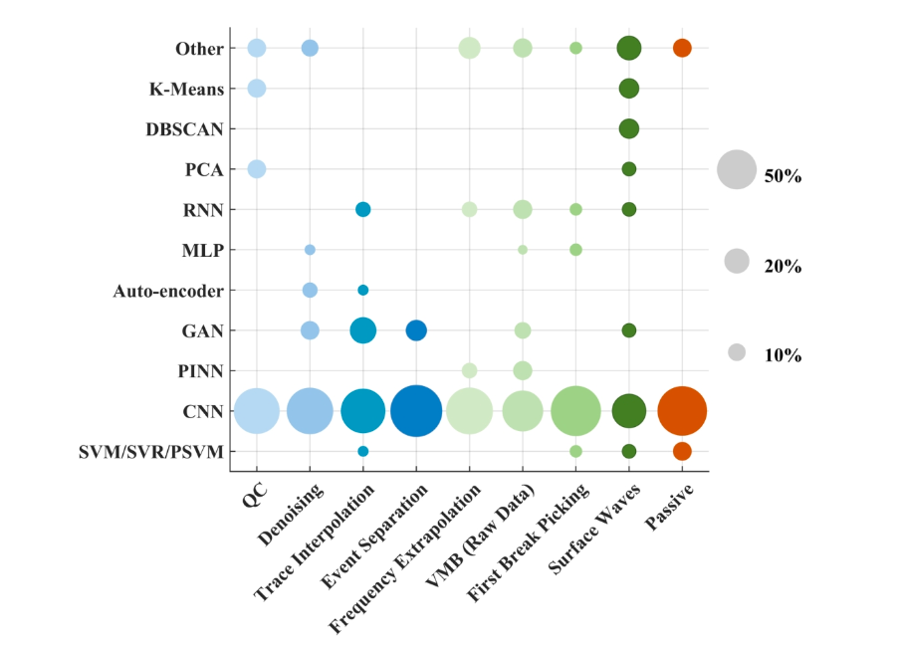
\includegraphics[width=0.8\textwidth]{Figure/Front_page/methods.png}
    \caption{\textit{Machine learning algorithms used for most prominent seismic processing applications \cite{khosro2023machine}}}
    \label{fig:methods}
\end{figure}



% \chapter{Comparison of interpolation methods}\label{ch:2}
% type here

% T-X domain

% F-X domain

% F-K domain

% T-domain Radon

% machine learning

\chapter{GAN Theory}\label{ch:3}
\section{Generative adversarial network}
Generative Adversarial Networks (GANs) represent a powerful class of deep learning models comprising generator(s) ($G$) and discriminator(s) ($D$). They are fully connected layers which often consist of deep convolutional neural networks (CNNs). \cite{siahkoohi2018seismic} $G$ generates synthetic samples from the embedding space while $D$ distinguishes between generated and real dataset samples. Through iterative training epochs, both $G$ and $D$ evolve by minimizing their respective losses, fostering the generation of more realistic samples by the generator.

\begin{figure}[H]
    \centering
    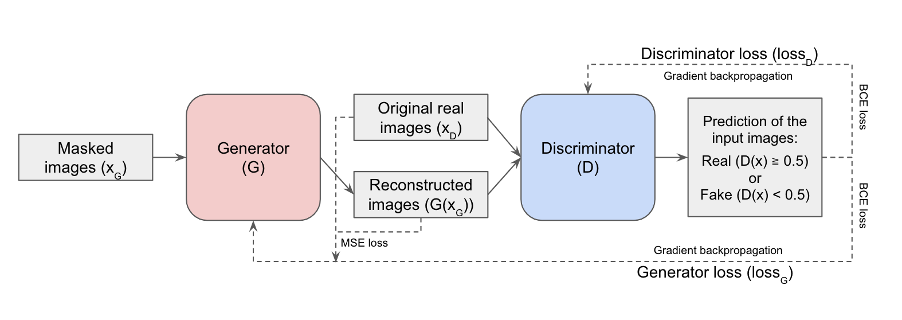
\includegraphics[width=\textwidth]{Figure/Front_page/flow chart.png}
    \caption{\textit{GAN architecture (modified from \cite{saxena2021generative})}}
    \label{fig:archi}
\end{figure}

\noindent In the context of image reconstruction, our application involves presenting $G$ with images containing missing columns, denoted as $x_{G}$, and obtaining interpolated images as the output, i.e., $G(x_{G})$. Subsequently, the discriminator $D$ assesses whether the given sample is a reconstructed image ($G(x_{G})$) or an authentic dataset image ($x_{D}$), assigning a scalar value between 0 (indicating a reconstructed image) and 1 (indicating a real dataset image). The generator loss ($loss_{G}$) is computed through a combination of binary cross-entropy (BCE) loss between $D(G(x_{G}))$ and 1, as well as mean squared error (MSE) loss between $G(x_{G})$ and $x_{D}$ (Equation \ref{eq:loss_G}). In contrast, the discriminator loss ($loss_{D}$) is determined by the sum of binary cross-entropy (BCE) loss between $D(x_{D})$ and 1, along with binary cross-entropy (BCE) loss between $D(G(x_{G}))$ and 0. (Equation 
 \ref{eq:loss_D}) The gradients of these losses are backpropagated to update the parameters of $G$ and $D$ \cite{saxena2021generative}.

\begin{equation}
loss_{G} = \underbrace{loss_{BCE}(D(G(x_{G})),1)}_\text{$G$ performance on producing synthetic image} + \underbrace{loss_{MSE}(G(x_{G}),x_{D})}_\text{Difference between synthetic and real image}
\label{eq:loss_G}
\end{equation}
\begin{equation}
loss_{D} = (\underbrace{loss_{BCE}(D(x_{D}),1)}_\text{$D$ performance on classifying real image} + \underbrace{loss_{BCE}(D(G(x_{G})),0)}_\text{$D$ performance on classifying synthetic image})/2
\label{eq:loss_D}
\end{equation}
 
\section{Neural network architecture}
Neural networks (NN) comprise interconnected layers of neurons, with various layer types (e.g., convolution, linear, and pooling) and activation functions (e.g., Rectified Linear Unit (ReLU), sigmoid, and tanh). The architecture's complexity impacts image reconstruction performance and computation time. Three neural network architectures have been investigated on our generator and discriminator, incorporating refined hyperparameters.

\begin{figure}[H]
    \centering
    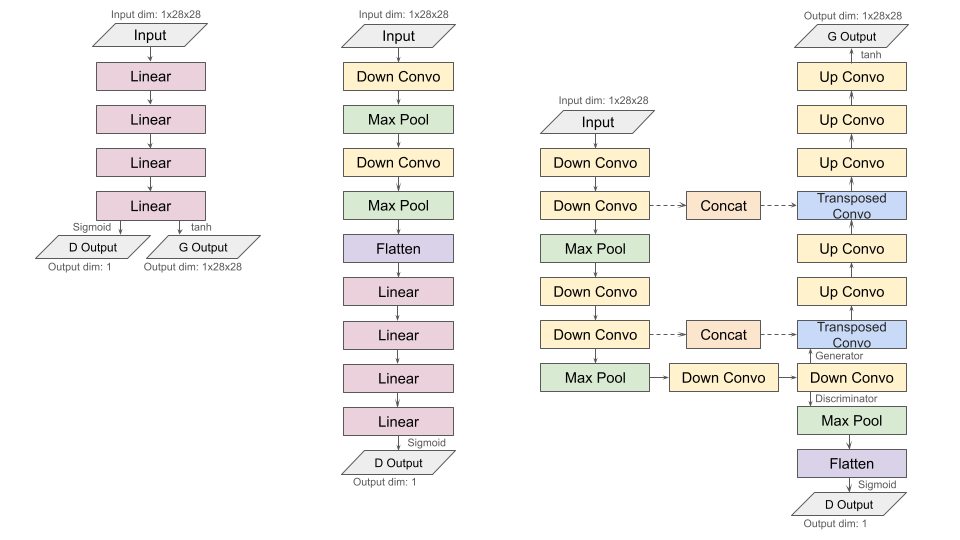
\includegraphics[width=\textwidth]{Figure/Front_page/Network architecture.png}
    \caption{\textit{Neural network architecture of linear layer model (left), LeNeT-5 (center) and U-NET (right)}}
    \label{fig:archi}
\end{figure}

\subsection{Linear layer model} \label{sub:linear}
This is the simplest model we built for this study, which consists of four linear transformations $y=xA^{T}+b$ and three ReLU functions. (Figure \ref{fig:archi} left) ReLU functions introduce non-linearity to NN, enabling them to learn complex tasks and mitigating the vanishing gradient problem. The generator employs linear layers with an increased output dimension, while the discriminator utilizes linear layers with a decreased output dimension.

\subsection{LeNeT-5}\label{sub:lenet}
Proposed in 1988, LeNet-5 stands as one of the earliest convolutional neural network (CNN) architectures \cite{lecun1998gradient}, notably designed for handwritten digit recognition. It is composed of two convolutional and pooling layers, a flattening function, four linear transformations, and three ReLU functions. (Figure \ref{fig:archi} center) 
Convolutional layers apply a kernel to each image pixel, capturing local patterns, while pooling layers retain the most relevant "summary" of features by downsampling the information. As LeNeT-5 down-samples the input dimension to 1, i.e. for classification purposes, we applied LeNet-5 only to our discriminator.

\subsection{U-NET}\label{sub:unet}
Introduced in 2015 by Olaf Ronneberger, Philipp Fischer, and Thomas Brox, U-NET is a convolutional neural network (CNN) architecture specifically designed for image segmentation tasks. Its distinctive U-shaped architecture comprises two key segments: the contracting path and the expanding path. \cite{ronneberger2015u, long2015fully}
\\\\
In our generator model, inspired by U-NET, the contracting path is implemented with six convolutional and two pooling layers. This configuration aims to decrease the spatial resolution of the input image while simultaneously increasing the number of feature channels. (Figure \ref{fig:archi} right) The contracting path is responsible for extracting essential features from the input image.
\\\\
Conversely, the expanding path in our model incorporates two transposed convolutional, five convolutional layers, and two concatenation layers.  (Figure \ref{fig:archi} right) This part of the network is designed to elevate the spatial resolution of the feature maps. Additionally, it combines these features with information from the contracting path to generate the final segmentation mask, using the concatenate functions.
\\\\
In our discriminator model, we leveraged the contracting path of the U-Net architecture, augmenting it with one pooling layer, one flattening function, and one linear layer. Our experimentation revealed that the U-Net architecture yielded the most refined interpolation results, which will be further discussed in chapter \ref{ch:4}.



\chapter{Experimental results and discussion}\label{ch:4}
\section{MNIST data experiment}
The MNIST (Modified National Institute of Standards and Technology) database comprises a collection of 60,000 training images and 10,000 testing images. These images represent handwritten digits and are digitally captured in a grayscale format, contained within a 28x28 pixel bounding box. \cite{deng2012mnist} To replicate the characteristics of the seismic traces interpolation problem, we adopted a strategy of masking 50\% of the columns in the images randomly. Subsequently, these partially masked images were fed into the generator. The generator, in turn, produced reconstructed images that effectively addressed the missing traces. 
\\\\
\noindent Three GAN architectures were utilized in this experiment. The Linear model incorporates a generator and discriminator, both constructed with the linear layer model (section \ref{sub:linear}). The LeNeT-5 model is composed of a generator using the linear layer model and a discriminator implemented with LeNeT-5 architecture (section \ref{sub:linear}). Additionally, the U-NET model integrates a generator based on U-NET and a discriminator constructed with a modified U-NET architecture (section \ref{sub:unet}).
\\\\
\noindent All three models underwent training using the Adam optimizer with a batch size of 64 and a learning rate of 0.0002. Dropout, with a probability of 0.5, was applied to both the generator and discriminator to enhance model generalization. The training ratio between the generator and discriminator was set to 2:1, emphasizing the importance of the generator's performance in image reconstruction. These parameter choices were meticulously chosen based on iterative experiments. Additional hyper-parameters for model training are detailed in the appendix table \ref{tab:param}.
\\\\
In Figure \ref{fig:mnist}, two generated samples are showcased. It is evident that the U-NET model produces results with the highest definition and bears the closest resemblance to the original images. The Linear model outputs a more generic representation of the digit along with a noisy background. The LeNeT-5 model performs between the aforementioned two models. Notably, in the example of the digit '4', both the Linear model and LeNeT-5 struggle to discern whether the masked image represents a '4' or '9', leading to a smudged reconstruction in the upper part of the image."

\begin{figure}[H]
    \centering
    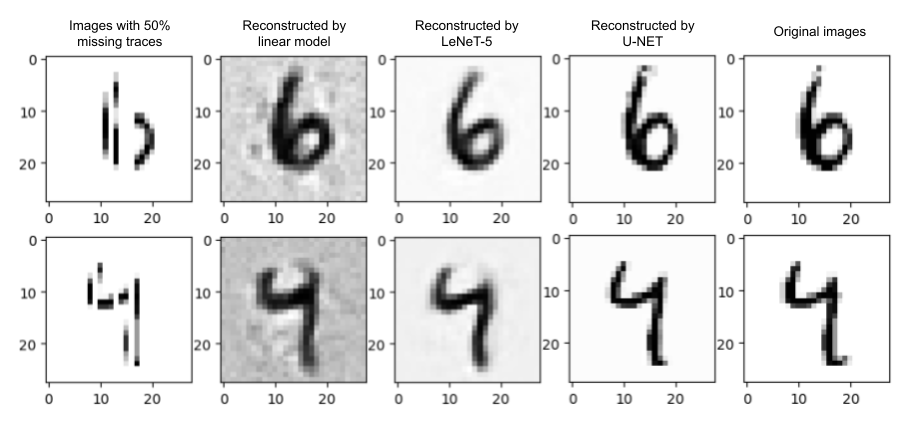
\includegraphics[width=\textwidth]{Figure/Front_page/mnist reconstruction.png}
    \caption{\textit{MNIST data reconstruction results comparison (from left to right: 50\% masked image, image reconstructed by the linear layer model, image reconstructed by LeNeT-5, image reconstructed by U-NET, original image) }}
    \label{fig:mnist}
\end{figure}

\section{F-MNIST data experiment}
Fashion-MNIST (F-MNIST) is a dataset comprised of Zalando's fashion article images. Each instance in the dataset is represented by a 28x28 pixel grayscale image, associated with a specific label from a set of 10 classes. These classes cover various fashion items, including shirts and sandals. \cite{xiao2017fashion} The dataset's size, GAN architectures, and hyper-parameters used in our experiment mirror those of the MNIST experiment. The only distinction lies in the training dataset, where Fashion-MNIST is employed.
\\\\
In Figure \ref{fig:fmnist}, the U-NET model exhibits superior performance in reconstructing intricate details of the clothing items. While LeNeT-5 demonstrates more refined edges compared to the Linear model, both models struggle to reproduce patterns on the shirt and accurately locate the straps on the sandal. Additionally, the reconstructed background in both cases appears noisy.

\begin{figure}[H]
    \centering
    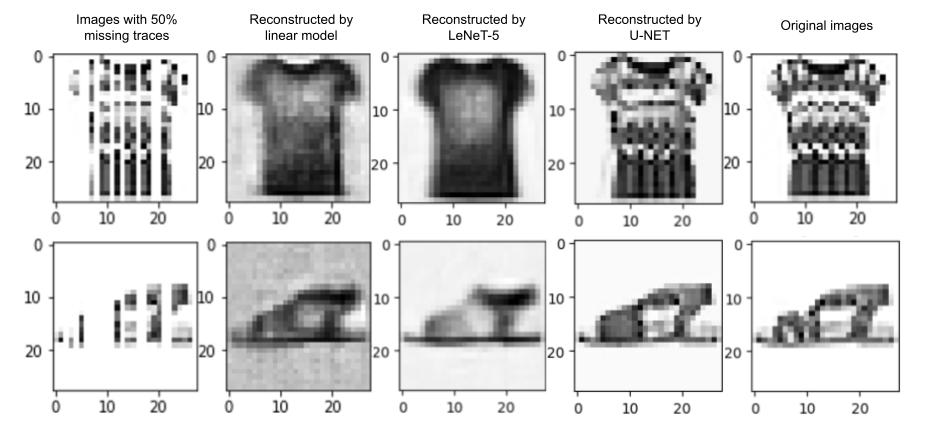
\includegraphics[width=\textwidth]{Figure/Front_page/fmnist reconstruction.png}
    \caption{\textit{Fashion-MNIST data reconstruction results comparison (from left to right: 50\% masked image, image reconstructed by the linear layer model, image reconstructed by LeNeT-5, image reconstructed by U-NET, original image)}}
    \label{fig:fmnist}
\end{figure}

\section{Discussion}
In Figures \ref{fig:mnist} and \ref{fig:fmnist}, we qualitatively assess the image reconstruction results. For a quantitative analysis, we examine the average loss per epoch of the GANs. The average discriminator losses converge to a value of 0.693, indicating that the generator produces replicas close enough to the original dataset to confuse the discriminator, i.e., the discriminator gives a guess of 0.5 for the input images. Substituting $D(x_{D}) = 0.5$ and $D(x_{G}) = 0.5$ into Equation \ref{eq:loss_D} yields a result of 0.693.
\\\\
The discriminator loss incorporates two binary cross-entropy (BCE) losses (equation \ref{eq:loss_D}), while the generator loss combines BCE loss and mean squared error (MSE) loss (equation \ref{eq:loss_G}). BCE losses are interdependent on the generator and discriminator within a model. To quantitatively evaluate the reconstruction results across models, we focus on the average generator MSE loss between the reconstructed and original images. 
\\\\
\noindent The training loss data indicates the models are well trained by the third epoch. (Figure \ref{fig:loss}) In the final epoch of MNIST validation, the average MSE losses are 0.0064, 0.0150, and 0.0213 for U-NET, LeNeT-5, and the Linear model, respectively. For F-MNIST training, the average MSE losses are 0.0065, 0.0162, and 0.0140. Excluding the Linear model, the average MSE loss is lower for the MNIST dataset, as handwritten digits contain fewer details than fashion items. U-NET outperforms the LeNeT-5 model by approximately 2.5 times. It's noteworthy that the computation time of U-NET is five times longer than LeNeT-5, with 7.18 seconds/iteration and 1.29 seconds/iteration, respectively, due to the increased complexity of the U-NET architecture. 
\\\\
\noindent The U-NET generator exhibits greater parameter efficiency, featuring 1,864,002 parameters compared to the Linear model generator's 14,631,184. Despite having an order of magnitude fewer parameters, the U-NET yields significantly superior results. This underscores that the linear model contains a considerable number of unnecessary parameters.
\\\\
\begin{figure}[H]
    \centering
    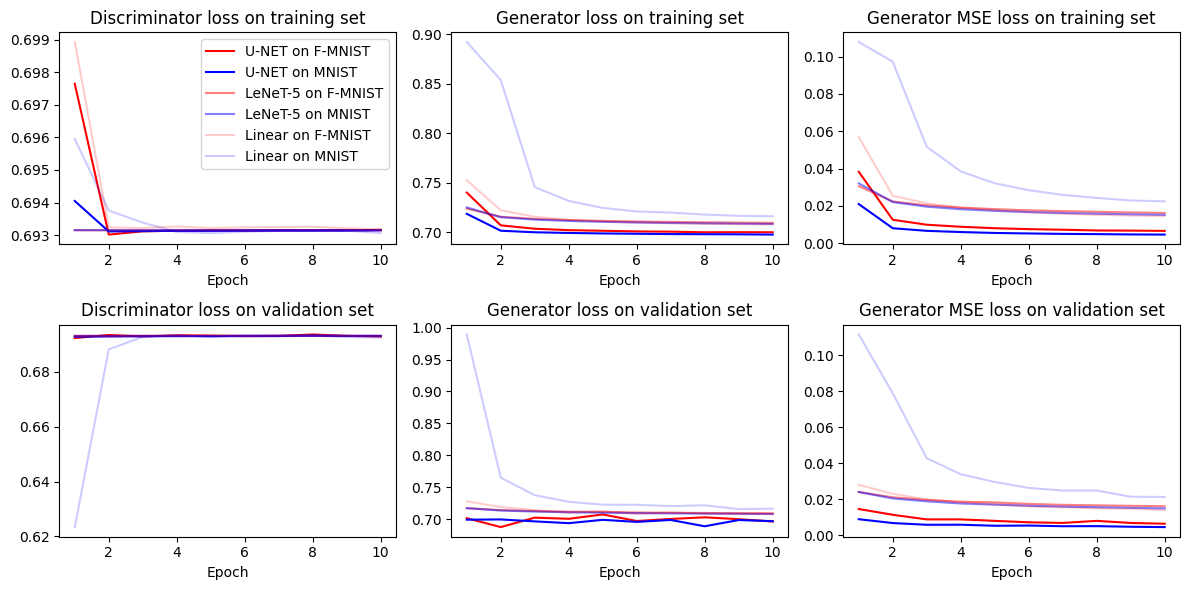
\includegraphics[width=\textwidth]{Figure/Front_page/losses.png}
    \caption{\textit{Average discriminator loss, generator loss, and generator MSE loss throughout 10 epochs for the three models on the MNIST and F-MNIST dataset}}
    \label{fig:loss}
\end{figure}

\noindent While GANs demonstrate satisfactory image reconstruction results, they are not without limitations. The first limitation is the challenge of training instability. Striking the right balance between the generator and discriminator poses difficulties, and GANs may experience oscillations or fail to converge during training. \cite{saxena2021generative} We raised the generator-discriminator training ratio to 2:1 to overcome this challenge. Second, there is the issue of feature loss due to missing information. The application of a masking function to random columns of the masked image can lead to areas with extended missing information, resulting in a blurred outcome (illustrated by the orange area in Figure \ref{fig:feature loss}). Third, GANs may encounter challenges in recovering high-frequency details. The struggle to capture intricate features, especially in small objects or complex patterns, can lead to potential smudging or loss of fine details during reconstruction (depicted by the red area in Figure \ref{fig:feature loss}).

% limitation
\begin{figure}[H]
    \centering
    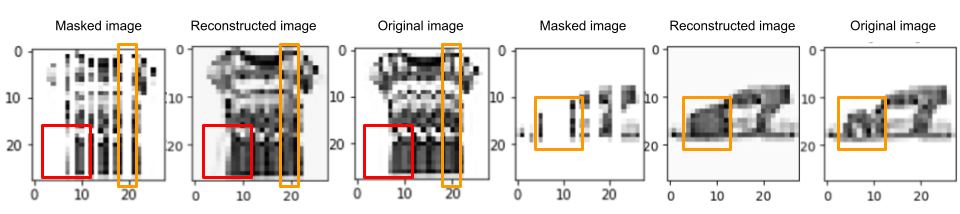
\includegraphics[width=\textwidth]{Figure/Front_page/feature lost.png}
    \caption{\textit{Feature loss in the reconstructed image due to missing information (orange) and high-frequency details (red)}}
    \label{fig:feature loss}
\end{figure}




\chapter{Conclusion}\label{ch:5}
In this study, we adopt a deep learning approach for seismic data interpolation, employing three GANs: U-NET, LeNet-5, and Linear model. We assess their performance in image reconstruction using simplified MNIST and F-MNIST datasets. The generators and discriminators, built with U-NET, LeNet-5, or Linear model, iteratively learn features between masked datasets and the original dataset over 10 training epochs, generating reconstructed images at varying resemblance levels. We compare GANs' interpolation results through qualitative examination of output features and quantitative assessment using MSE losses on validation sets. U-NET consistently yields the most refined and accurate reconstruction, while LeNet-5 and Linear model capture the general shapes of handwritten digits and fashion items. Looking ahead to seismic data interpolation, we anticipate GANs to provide satisfactory results with more complex neural network architectures and fine-tuning of hyper-parameters. GANs offer flexibility by not requiring any velocity models or relying on linearity/sparsity assumptions. However, challenges such as training instability, feature loss due to missing information, and high-frequency details recovery need to be addressed.
\\\\
In future research, we plan to extend our GANs interpolation approach to seismic datasets. An exploratory avenue would involve experimenting with CycleGANs, potentially incorporating U-NET with additional layers for enhanced performance. Additionally, exploring different masking schemes, such as determining the maximum consecutive columns to be masked while retaining features, could provide valuable insights into improving overall performance.

% \chapter{Appendix}\label{ch:6}
% \chapter{Data management plan}

The datasets utilized in this study are sourced from the PyTorch dataset library, \textit{torchvision.datasets.MNIST()} for MNIST datasets and \textit{torchvision.datasets.FashionMNIST()} for Fashion-MNIST datasets. Training and validation sets are imported separately. The Jupyter notebooks for model training, namely \textbf{gan\_interpolate\_linear.ipynb, gan\_interpolate\_lenet.ipynb, gan\_interpolate\_unet.ipynb}, are available on GitHub, along with the plotting notebook \textbf{gan\_plots.ipynb}. To reproduce the interpolation results using the same masked image, one can utilize the .pth files in the \textbf{sample\_pics} directory. The PyTorch version used is v2.2.1, and the code was written in Python v3.9.2.


\chapter{Appendix}
\begin{table}[H]
    \centering
    \begin{tabular}{ll}
    \hline
    \textbf{Parameter}            &  \textbf{value}       \\
    \hline
    Batch size & 64 \\
    Masking rate & 0.4 \\
    Learning rate & 0.0002 \\
    Number of epochs & 10 \\
    Dropout & 0.5 \\
    Optimiser & Adam \\
    Training ratio & 2 Generator / 1 Discriminator \\
    
    \hline
    \end{tabular}
    \caption{\textit{Hyper-parameters for model training}}
    \label{tab:param}
\end{table}

% Batch size: 64
% Masking rate: 0.4
% Learning rate: 0.0002
% Number of epoch: 10
% Generator: Simple linear layers (4 layers)
% Discriminator: Simple linear layers (4 layers)
% Optimiser: Adam
% Loss: BCELoss
% Training ratio: 1 Generator /1 Disciminator
% Training time: 10m 40s (10 epochs 64 batch size)


\begin{figure}[H]
    \centering
    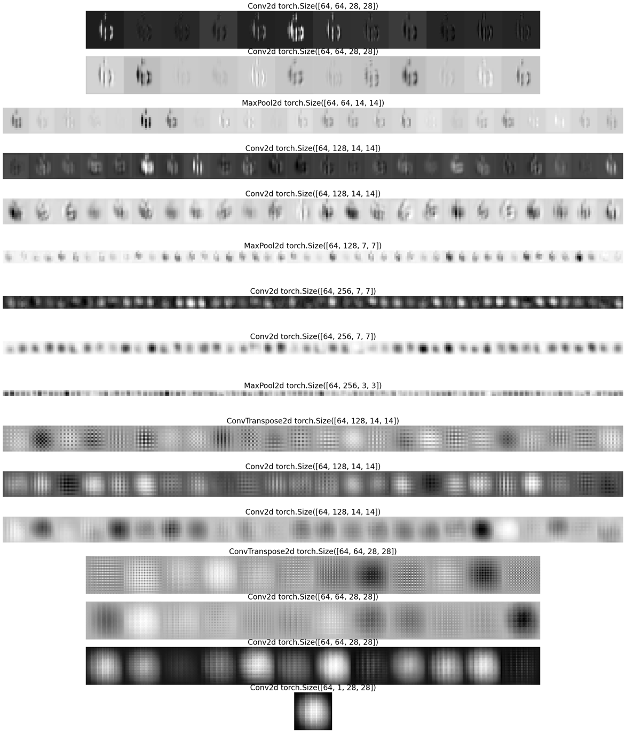
\includegraphics[width=\textwidth]{Figure/Front_page/mnist feature map.png}
    \caption{\textit{U-NET feature map for MNIST input}}
    \label{fig:mnist feature loss}
\end{figure}

\begin{figure}[H]
    \centering
    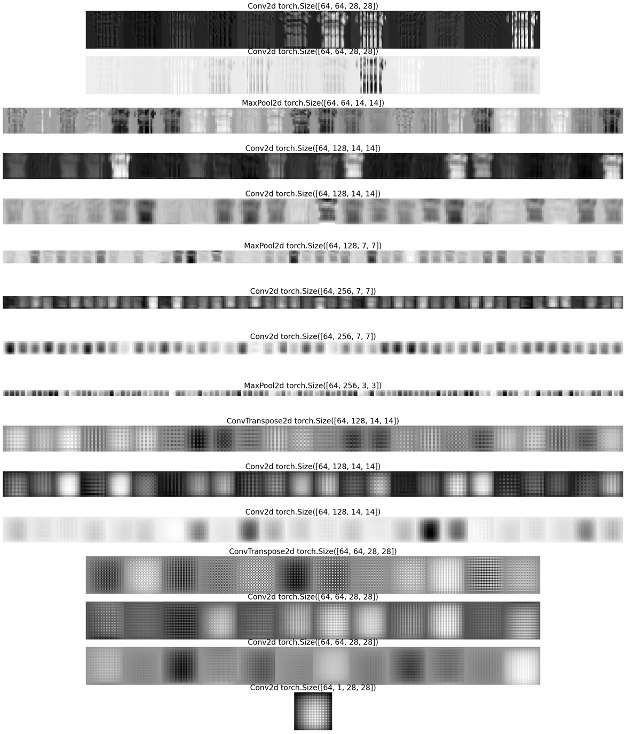
\includegraphics[width=\textwidth]{Figure/Front_page/fmnist feature map.png}
    \caption{\textit{U-NET feature map for F-MNIST input}}
    \label{fig:fmnist feature map}
\end{figure}

\appendix
\chapter{Data management plan}

The datasets utilized in this study are sourced from the PyTorch dataset library, \textit{torchvision.datasets.MNIST()} for MNIST datasets and \textit{torchvision.datasets.FashionMNIST()} for Fashion-MNIST datasets. Training and validation sets are imported separately. The Jupyter notebooks for model training, namely \textbf{gan\_interpolate\_linear.ipynb, gan\_interpolate\_lenet.ipynb, gan\_interpolate\_unet.ipynb}, are available on GitHub, along with the plotting notebook \textbf{gan\_plots.ipynb}. To reproduce the interpolation results using the same masked image, one can utilize the .pth files in the \textbf{sample\_pics} directory. The PyTorch version used is v2.2.1, and the code was written in Python v3.9.2.


\chapter{Appendix}
\begin{table}[H]
    \centering
    \begin{tabular}{ll}
    \hline
    \textbf{Parameter}            &  \textbf{value}       \\
    \hline
    Batch size & 64 \\
    Masking rate & 0.4 \\
    Learning rate & 0.0002 \\
    Number of epochs & 10 \\
    Dropout & 0.5 \\
    Optimiser & Adam \\
    Training ratio & 2 Generator / 1 Discriminator \\
    
    \hline
    \end{tabular}
    \caption{\textit{Hyper-parameters for model training}}
    \label{tab:param}
\end{table}

% Batch size: 64
% Masking rate: 0.4
% Learning rate: 0.0002
% Number of epoch: 10
% Generator: Simple linear layers (4 layers)
% Discriminator: Simple linear layers (4 layers)
% Optimiser: Adam
% Loss: BCELoss
% Training ratio: 1 Generator /1 Disciminator
% Training time: 10m 40s (10 epochs 64 batch size)


\begin{figure}[H]
    \centering
    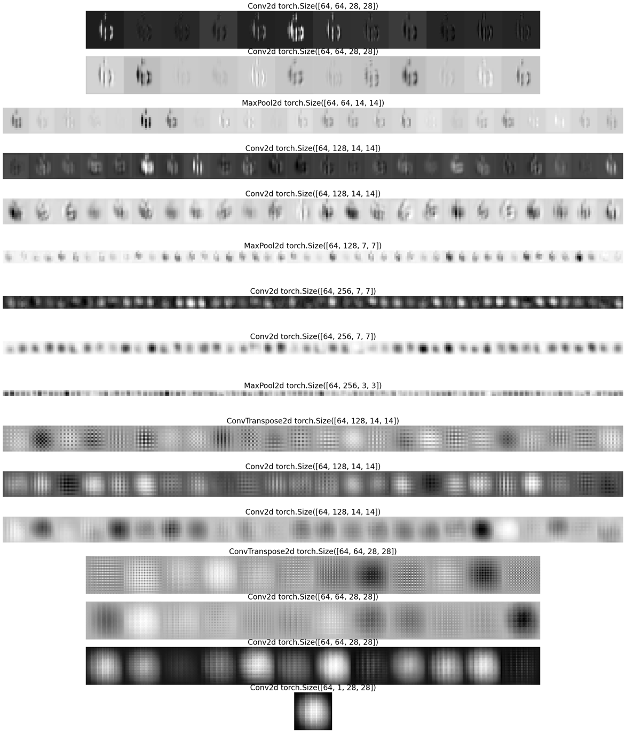
\includegraphics[width=\textwidth]{Figure/Front_page/mnist feature map.png}
    \caption{\textit{U-NET feature map for MNIST input}}
    \label{fig:mnist feature loss}
\end{figure}

\begin{figure}[H]
    \centering
    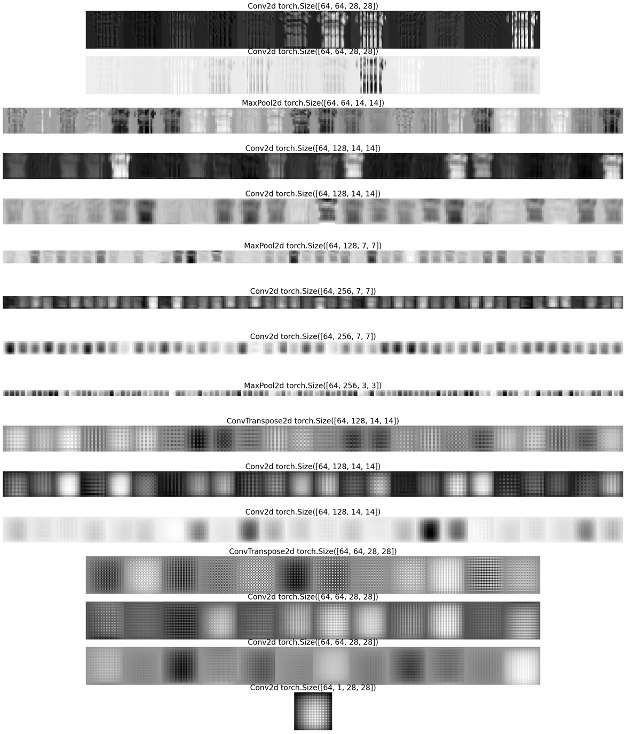
\includegraphics[width=\textwidth]{Figure/Front_page/fmnist feature map.png}
    \caption{\textit{U-NET feature map for F-MNIST input}}
    \label{fig:fmnist feature map}
\end{figure}

\newpage
\bibliographystyle{apacite}
\addcontentsline{toc}{chapter}{Bibliography}
\bibliography{bibliography.bib}
\end{document}